\section{Durchführung}
\label{sec:Durchführung}

Für den Versuch wird ein in \autoref{fig:Acrylblock} dargestellter Quaderförmiger Acrylblock verwendet,
in dem elf Fehlstellen in Form von Bohrungen eingearbeitet sind.
Im ersten Schritt wird die Höhe des Acrylblocks sowie die sämtlicher Bohrungen mit der Schieblehre gemessen.
Auch der Durchmesser der Löcher wird vermessen, die Werte dienen später als Referenz für die Ultraschallmessungen.
\begin{figure}
    \centering
    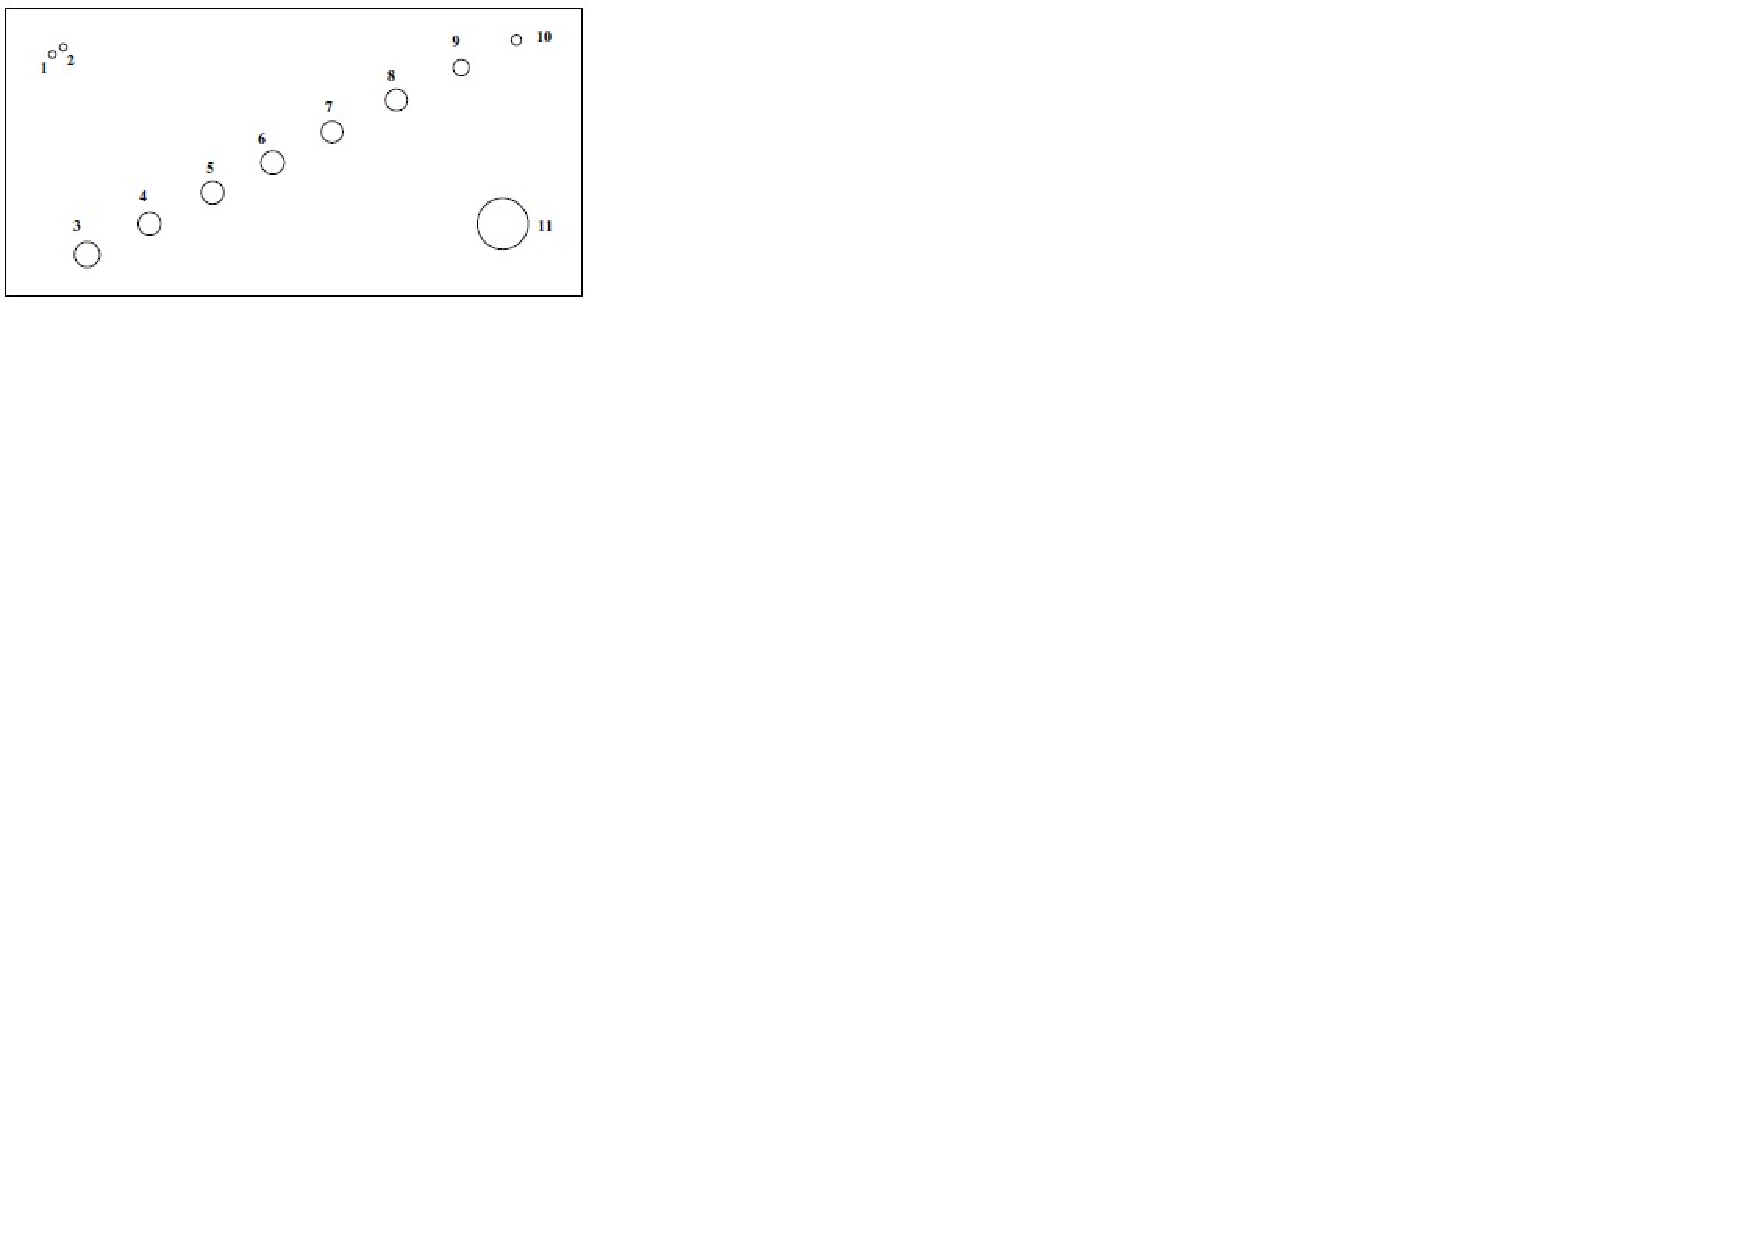
\includegraphics[height=4cm]{content/pics/acrylblock.pdf}
    \caption{Skizze des verwendeten Acrylblocks.\cite{US2}}
    \label{fig:Acrylblock}
\end{figure}

\subsection{Bestimmung der Schallgeschwindigkeit und Dicke der Kopplungsschicht}
Im ersten Versuchsteil werden 7 Löcher verwendet, um mithilfe eines \textit{A-Scans} die Laufzeit des Impulses
bis zu deren Position zu bestimmen. Zusammen mit den vorher gemessenen Positionen der Löcher kann anschließend
die Schallgeschwindigkeit bestimmt werden.

\subsection{Vermessung der Fehlstellen mithilfe eines \textit{A-Scans}}
\label{sec:arschscan}
Im Computerprogramm wird nun die theoretische Schallgeschwindigkeit in Acryl
$c_{\symup{theorie}}=\qty{2730}{\metre\per\second}$ \cite{c_Acryl} ergänzt, dies ermöglicht dem Programm
die gemessenen Laufzeiten direkt als Längen anzugeben.
Unter Verwendung eines \textit{A-Scans} werden alle zuvor händisch bestimmten Maße nun erneut genommen,
indem der Block von der Ober- und Unterseite gescannt wird.
Dies ermöglicht zusätzlich, den Durchmesser der Bohrungen mithilfe der Ultraschalltechnik zu berechnen.

\subsection{Untersuchung des Auflösungsvermögens}
Um mögliche Unterschiede des Auflösungsvermögens bei Verwendung verschiedener Frequenzen der Ultraschallwellen
zu untersuchen, werden zwei benachbarte Bohrungen betrachtet. Die selbe Stelle wird mit einer $\qty{1}{\mega\hertz}$
sowie mit einer $\qty{2}{\mega\hertz}$ Sonde gescannt. Zur Feststellung möglicher Unterschiede werden die ausgegebenen
Grafiken verglichen.

\subsection{Vermessung der Fehlstellen mithilfe eines \textit{B-Scans}}
Analog zu \autoref{sec:arschscan} werden die Fehlstellen wieder Vermessen, jedoch
wird nun der \textit{B-Scan} eingesetzt. Die Positionen der Bohrungen können hierbei aus den Grafiken abgelesen werden,
die Durchmesser lassen sich wieder aus den Differenzen bestimmen.

\subsection{Untersuchung eines Brustmodells auf Tumore}
Zuletzt soll ein Brustmodell mit einem \textit{B-Scan} auf Tumore untersucht werden. Dafür wird deren Position
zuerst ertastet, um die ungefähre Position für den Ultraschallscan zu kennen.
Anschließend wird der \textit{B-Scan} durchgeführt und graphisch ausgewertet, um die Existenz und Position
der Tumore zu verifizieren.